\section{Filtro 1: Blur}

\subsection{Explicacion}
El filtro de blur se aplica en cada pixel de la imagen exceptuando los del borde, para eso tomamos el pixel a modificar y los 8 adyacentes y los promediamos para obtener el valor final del pixel.

Debemos tener cuidado a la hora de procesar la imagen de no pisar los datos y operar con los pixeles de la imagen original a la hora de hacer las cuentas.

\subsection{Implementacion 1}
La primera implementacion nos pide que trabajemos de a 1 pixel por iteracion.

Los pixeles estan compuestos por 4 bytes: A R G B, esto nos permite cargar de memoria en un registro XMM 4 pixeles, como nosotros necesitamos 9 pixeles en 3 filas de pixeles diferentes vamos a necesitar 3 registros XMM para cargar los pixeles (Para esto usamos los registros XMM0, XMM2 y XMM4). Y ademas necesito 3 registros XMM mas para luego desenpaquetar los bytes a words. \\

Ademas necesitaremos 6 registro de proposito general: \\
RDI que lo usamos para iterar sobre el eje X \\
R9 que lo usamos para iterar sobre y \\
R12 que es un puntero a la copia de la fila superior \\
R13 que es un puntero a la copia de la fila actual \\
R8 es un puntero a la inferior fila \\
R10 es un puntero a la fila actual de la imagen (fila que estoy modificando) \\

\begin{figure}[h!]
	\centering
	\includegraphics[scale=0.5]{images/BlurASM1_0}
\end{figure}

Antes de comenzar el ciclo incicializo R9 en 2 y posiciono el puntero a la imagen en la segunda fila de pixeles.

Al principio de cada ciclo de y muevo R8 a R10, aumento R8 en una fila y inicializo el iterador en x (RDI) en 0.

Muevo a los registros los 3 grupos de pixeles. \\
	XMM0 = [R12 + RDI] = xx ; p2 ; p1 ; p0 \\
	XMM1 = [R13 + RDI] = xx ; p5 ; p4 ; p3 \\
	XMM2 = [R8  + RDI] = xx ; p8 ; p7 ; p6 \\
\\
Despues desenpaqueto los pixeles de byte a word para poder sumar los 9 pixeles sin saturacion, hacemos una copia de cada uno para poder desenpaquetar la parte inferior en un registro y la superior en otro (XMM1 = XMM0, XMM3 = XMM2, XMM5 = XMM4) y ademas llenamos un registro (XMM15) con ceros para expandir los componentes con ceros.
Una vez desenpaquetados nos quedan los registros con los siguientes valores.
\\
	XMM0 = p1 ; p0 \\
 	XMM1 = xx ; p2 \\
 	XMM2 = p4 ; p3 \\
	XMM3 = xx ; p5 \\ 
	XMM4 = p7 ; p6 \\
	XMM5 = xx ; p8 \\
\\
Ahora sumamos los registros y luego hacemos la division. \\
Sumando XMM0, XMM2 y XMM3 en XMM15 \\
	XMM15 = p1 + p4 + p7 ; p0 + p3 + p6	\\
Sumando XMM1, XMM3 y XMM4 en XMM14	\\
	XMM14 = x ; p2 + p5 + p8 \\
Ahora hago una copia de XMM15 en XMM13 y la shifteo 8 bytes a la derecha \\
	XMM13 = x ; p1 + p4 + p7 \\
Por ultimo sumo XMM15, XMM14 y XMM13 en XMM15 \\
	XMM15 x ; p0 + p1 + p2 + p3 + p4 + p5 + p6 + p7 + p8 \\

Para hacer la division optamos por multiplicar por $(2^{16} / 9) + 1$ y luego shiftear 16 bits a la derecha cada componente. Para eso tengo el valor por el cual voy a multiplicar en memoria precalculado, al principio del programa decido guardarlo en XMM12.
Hago una copia de XMM15 en XMM14 y multiplico por XMM12 guardandome la parte superior de la mutiplicacion en XMM15 y la inferior en XMM14. Luego empaqueto los dos valores juntos como doubleword y los guardo en XMM14 y shifteo a 16 a la derecha.
Por ultimo empaqueto los valores obtenidos como words y luego como bytes y los guardo en la posicion de memoria del pixel actual.

Aumento en 4 el iterador en x y comparo con el tamaño en bytes de una linea de pixeles, si es menor itero nuevamente en x.

Si es mayor o igual voy a hacer 2 copias de las lineas de pixeles siguientes (Que necesito para operar la siguiente fila).

\subsection{Implementacion 2}
La implementacion 2 nos pide trabajar de a 4 pixeles por iteracion.

Para eso voy a calcular primero los pixeles P0 y P1, y despues el P2 y P3 tratando de minimizar la cantidad de accesos a memoria. \\

\begin{figure}[h!]
	\centering
	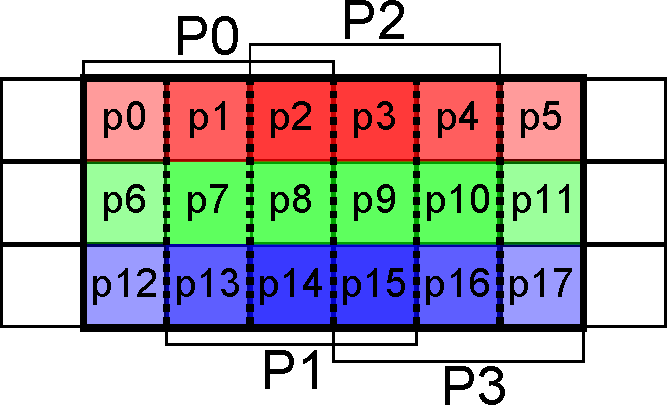
\includegraphics[scale=0.5]{images/BlurASM2_1}
\end{figure}

Para hacer los calculos vamos a tomar 6 set de 4 pixeles que nos permiten sumar en un solo registro 2 pixeles al mismo tiempo usando solo sumas, cada set ira adentro de un registro XMM. Ademas se necesitan 6 registros XMM mas para poder desenpaquetar los bytes a words y asi no tener saturacion. \\

Al igual que la implementacion uno necesitaremos los mismos 6 registros de proposito general. \\

\begin{figure}[h!]
	\centering
	\includegraphics[scale=0.5]{images/BlurASM2_0}
\end{figure}

Antes de comenzar el ciclo iniciamos el iterador en y (R9) y posicionamos el puntero a la imagen en la segunda fila de pixeles. \\

Al igual que en la primera implementacion nos guardamos una copia del puntero a la fila que vamos a incrementar y movemos R8 a la siguiente fila de pixeles. Ademas inicializamos el iterador de X (RDI) en 0. \\

Muevo a los registros los 6 pixeles. \\
	XMM0 = p3 ; p2 ; p1 ; p0 \\
	XMM2 = p4 ; p3 ; p2 ; p1 \\
	XMM4 = p9 ; p8 ; p7 ; p6 \\
	XMM6 = p10 ; p9 ; p8 ; p7 \\
	XMM8 = p15 ; p14 ; p13 ; p12 \\
	XMM10 = p16 ; p15 ; p14 ; p13 \\
\\
Al igual que en la implementacion uno desenpaquetamos los registros haciendo una copia y desenpaquetando la parte superior en el registro original y la inferior en la copia. Para desenpaquetar uso un registro con ceros (XMM15) \\
	XMM0 = p1 ; p0 \\
 	XMM1 = p3 ; p2 \\
 	XMM2 = p2 ; p1 \\
	XMM3 = p4 ; p3 \\ 
	XMM4 = p7 ; p6 \\
	XMM5 = p9 ; p8 \\
	XMM6 = p8 ; p7 \\
 	XMM7 = p10 ; p9 \\
 	XMM8 = p13 ; p12 \\
	XMM9 = p15 ; p14 \\ 
	XMM10 = p14 ; p13 \\
	XMM11 = p16 ; p15 \\
\\
Ahora sumo los registros XMM0, XMM1, XMM2, XMM4, XMM5, XMM6, XMM8, XMM9, XMM10 uno por uno con XMM15, al terminar XMM15 = p1 + p2 + p3 + p7 + p8 + p9 + p13 + p14 + p15 ; p0 + p1 + p2 + p6 + p7 + p8 + p12 + p13 + p14, esto como se ve en la imagen es igual a P1 | P0. \\

Ahora hago la division de cada pixel igual que en la primera implementacion, antes de dividir me guardo una copia de XMM15 en XMM0, divido por 9 y luego shifteo 8 bytes a la derecha y divido nuevamente. \\

Luego muevo los pixeles procesados P0 y P1 a memoria, posicionandolos con el offset correcto. \\

Ahora para procesar los pixeles P2 y P3 muevo 3 grupos mas de pixeles de la memoria a los registros XMM0, XMM4 y XMM8. \\
	XMM0 = p5 ; p4 ; p3 ; p2 \\
	XMM4 = p11 ; p10 ; p9 ; p8 \\
	XMM8 = p17 ; p16 ; p15 ; p14 \\
\\
Ademas hago copias en XMM1, XMM5 y XMM9 y desenpaqueto de byte a word. \\
	XMM0 = p3 ; p2 \\
 	XMM1 = p5 ; p4 \\
	XMM4 = p9 ; p8 \\
	XMM5 = p11 ; p10 \\
 	XMM8 = p15 ; p14 \\
	XMM9 = p17 ; p16 \\
\\
Nuevamente sumo los registros XMM0, XMM1, XMM3, XMM4, XMM5, XMM7, XMM8, XMM9, XMM11 uno por uno con XMM15, XMM15 = p3 + p4 + p5 + p9 + p10 + p11 + p15 + p16 + p17 ; p2 + p3 + p4 + p8 + p9 + p10 + p14 + p15 + p16, esto es P3 | P2. \\

Hago la division al igual que arriba y guardo los pixeles procesados P2 y P3 en memoria. \\

Comparo el iterador con la cantidad de pixeles en una fila y repito hasta que llegue hasta los ultimos 16 bytes de la fila, en los ultimos 16 bytes me fijo de cargarlos en memoria en solo 3 registros XMM y procesarlos al igual que la primera parte del ciclo para asegurarme de no pasarme. \\

Al final del ciclo hago las copias, incremento el iterador de filas y checkeo si llegue al final. \\

\subsection{Resultados}
La primera experimentacion que hicimos es correr las 3 implementaciones (C compilada con optimizaciones de nivel 3) con la imagen de lena en diferentes tamaños (multiplos de 16x16, hasta 320x320), corrimos 10 test con cada tamaño y luego promediamos los valores para reducir la cantidad de ruido. \\

\begin{figure}[h!]
	\centering
	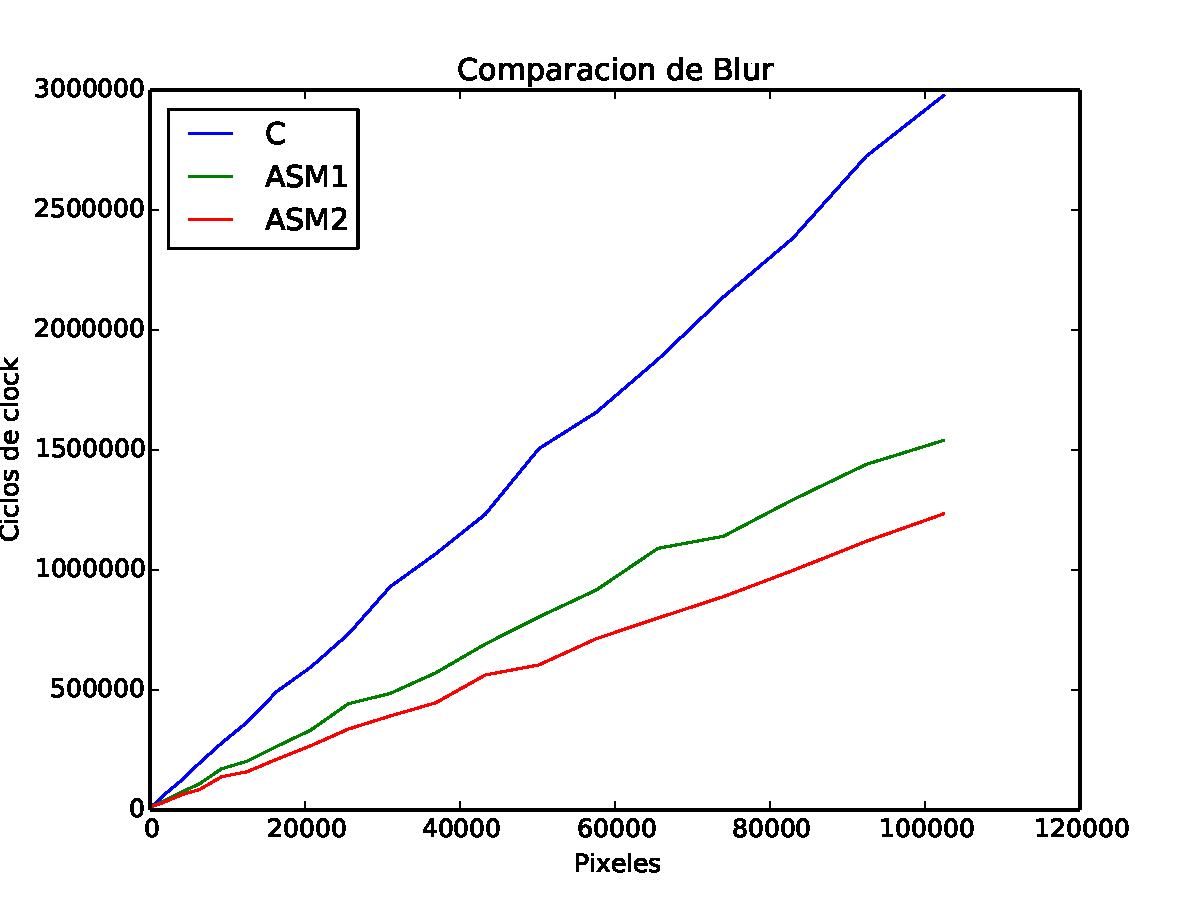
\includegraphics[scale=0.5]{images/blur_comp}
\end{figure}

Este grafico nos muestra que el codigo de ASM2 pareceria ser el mas rapido. Antes de confirmar esto queremos ver que no haya ningun tipo de factor que beneficie a ASM2. \\

\begin{figure}[h!]
	\centering
	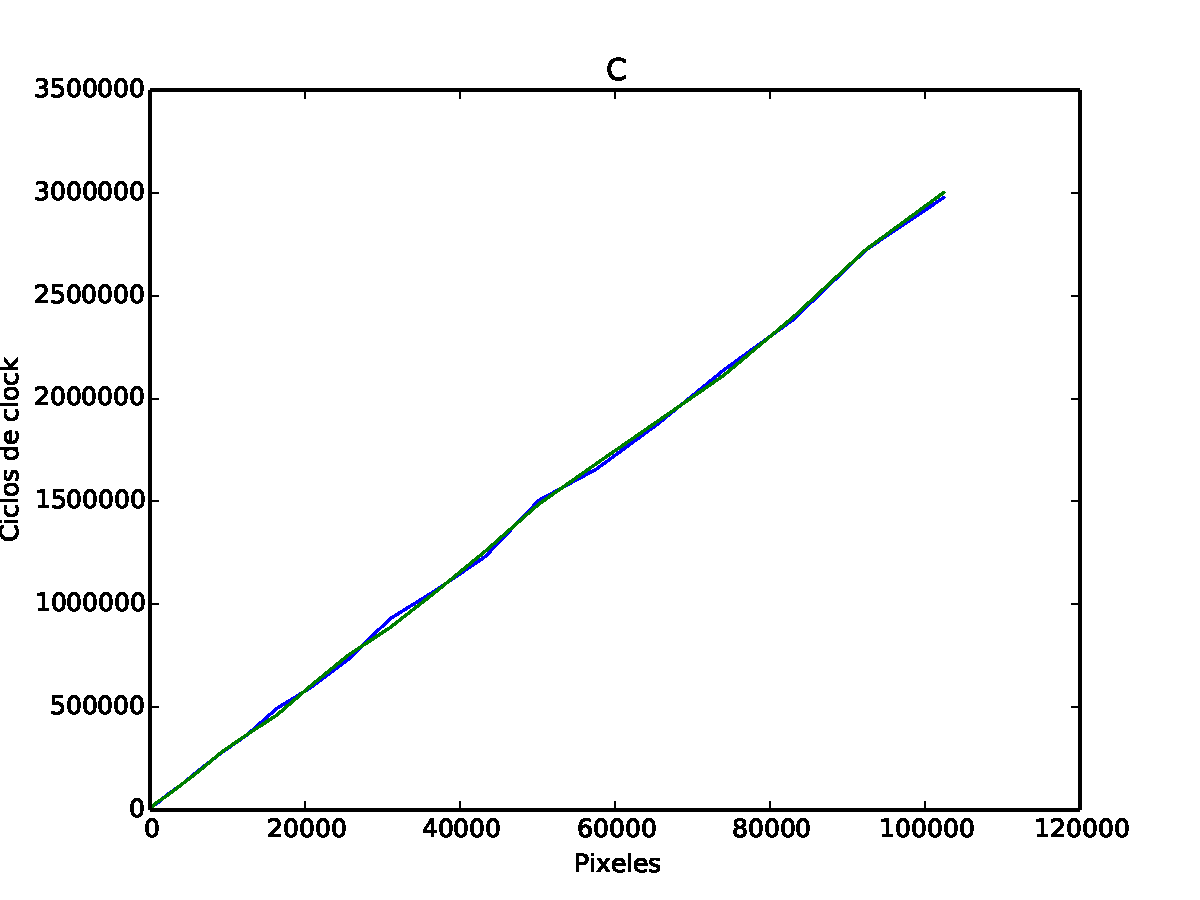
\includegraphics[scale=0.28]{images/c_blur_lena}
	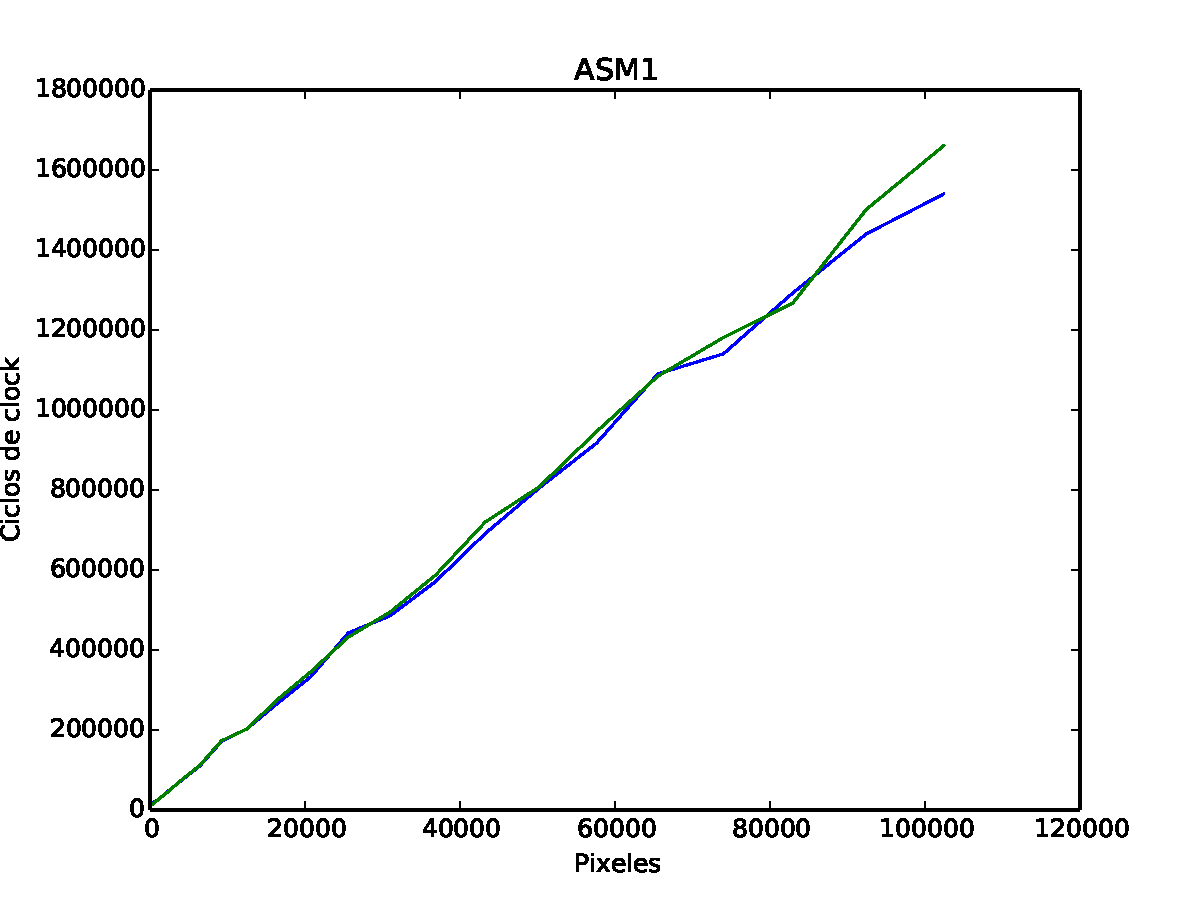
\includegraphics[scale=0.28]{images/asm1_blur_lena}
	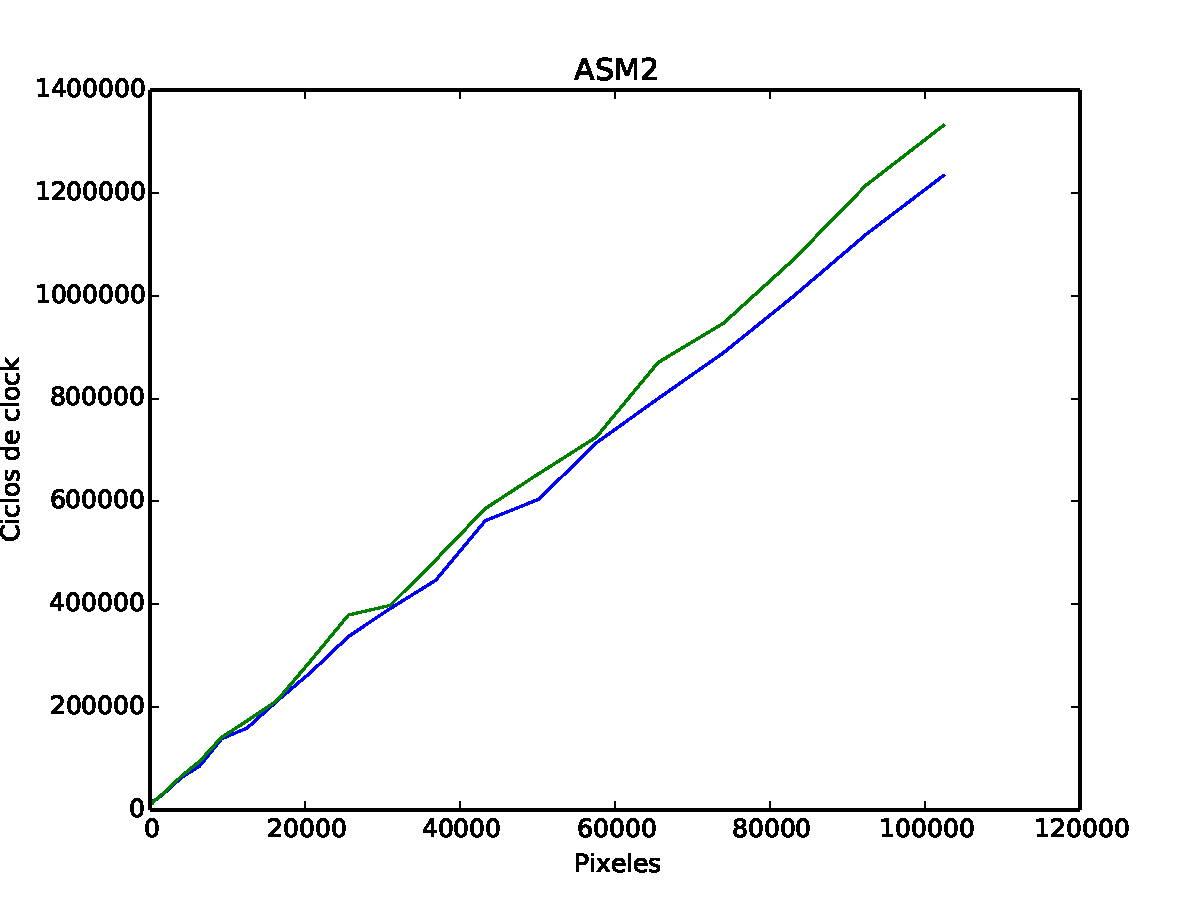
\includegraphics[scale=0.28]{images/asm2_blur_lena}
\end{figure}

Tanto en el codigo de C como en el ASM1 y ASM2 no poseen ningun salto condicional que dependa de 

\subsection{Conclusion}